\documentclass[a4paper,12pt]{article}
\usepackage[utf8]{inputenc}
\usepackage[russian]{babel}
\usepackage{amsmath, amsfonts, amssymb}
\usepackage{geometry}
\usepackage{booktabs}
\usepackage{caption}
\usepackage{hyperref}
\usepackage{graphicx}

\usepackage{minted}
\usemintedstyle{colorful}

\geometry{left=2cm,right=2cm,top=2cm,bottom=2cm}
\hypersetup{colorlinks=true, linkcolor=black, urlcolor=blue}

\begin{document}
\begin{titlepage}
    \centering
    Федеральное государственное автономное образовательное учреждение высшего образования «Национальный исследовательский университет ИТМО» \\
    \vspace{1cm}
    Факультет Программной Инженерии и Компьютерной Техники \\
    \vfill
    {\large «Системы искусственного интеллекта»} \\
    \vspace{0.5cm}
    Лабораторная работа №2 \\
    Логистическая регрессия \\
    \vfill
    \vspace{\fill}
    \begin{flushright}
        \textbf{Выполнил:} \\
        Козаченко Данил Александрович \\
        \textbf{Группа P3312} \\
        \textbf{Проверила:} \\
        Болдырева Елена Александровна
    \end{flushright}
    \vspace{2cm}
    Санкт-Петербург
    2026г.
\end{titlepage}


\begin{centering}
    \renewcommand{\contentsname}{Содержание}
    \tableofcontents
\end{centering}
\newpage

\section{Введение}

Цель работы - реализовать логистическую регрессию с нуля и исследовать влияние гиперпараметров на классификацию пассажиров Титаник по признаку выживания. Целевая переменная \texttt{Survived} принимает значения 0 (не выжил) и 1 (выжил).

Выполнены загрузка и предобработка данных, численная и графическая оценка статистики, разбиение на обучающую и тестовую части, реализация сигмоиды, функции потерь и обучения. Исследованы шаг обучения, число итераций и два оптимизатора: градиентный спуск и метод Ньютона

\section{Описание метода}

Для бинарной целевой переменной используется модель Бернулли с вероятностью успеха $p_i$. Логистическая регрессия связывает эту вероятность с линейным предиктором:
\[
 z_i=x_i^Tw,\qquad p_i=\sigma(z_i)=\frac{1}{1+e^{-z_i}},
 \qquad \log\frac{p_i}{1-p_i}=x_i^Tw.
\]

Максимизация правдоподобия Бернулли эквивалентна минимизации средней log loss:
\[
 L(w)=-\frac1n\sum_{i=1}^{n}\bigl[y_i\log p_i+(1-y_i)\log(1-p_i)\bigr].
\]

Сигмоида вычисляется отдельно для положительных и отрицательных аргументов, что исключает переполнение экспоненты.

Обозначая матрицу признаков со свободным членом через $X$, получаем:
\[
 g=\nabla L=\frac{X^T(p-y)}n,\qquad
 H=\frac{X^T\operatorname{diag}(p_i(1-p_i))X}n.
\]
Градиентный спуск (GD) обновляет $w\leftarrow w-\alpha g$, метод Ньютона - $w\leftarrow w-\alpha H^+g$. Псевдообратная матрица $H^+$ вычисляется средствами NumPy и позволяет обработать вырожденный гессиан. Для Ньютона $\alpha$ задаёт долю полного шага.

Все веса изначально равны нулю, регуляризация отсутствует. Обучение заканчивается по достижении \texttt{max\_iter} обновлений или при $\|g\|_\infty\leq10^{-8}$. В таблицах различаются максимальное и фактическое числа итераций

\section{Псевдокод метода}

Общая схема реализованных алгоритмов:
\begin{minted}[fontsize=\small,breaklines]{text}
Read train.csv
Describe raw data and plot statistics

Split rows: train/test = 80/20,

Fit numeric medians, means, scales and categories on train
Transform train and test using the same fitted parameters
For optimizer in {GD, Newton}:
  For alpha in {0.01, 0.1, 0.5, 1.0}:
    For max_iter in {10, 100, 1000}:
      Add intercept column; initialize w = 0
      Repeat at most max_iter times:
        p = sigmoid(X_train @ w)
        g = X_train.T @ (p - y_train) / n
        If max(abs(g)) <= 1e-8: stop
        If GD: direction = g
        If Newton:
          H = X_train.T @ diag(p*(1-p)) @ X_train / n
          direction = pinv(H) @ g
        w = w - alpha * direction
        Record training log loss
      Predict test probabilities and classes (threshold = 0.5)
      Compute accuracy, precision, recall, F1 and log loss
      Save actual iteration count, convergence flag and time
Compare all combinations on the same test rows
\end{minted}

\section{Результаты выполнения}

В \texttt{titanic/train.csv} содержится 891 пассажир и 12 столбцов, включая целевую переменную. Не выжил 549 пассажиров, выжили 342 (38.38\%).

\begin{table}[H]
\centering
\caption{Описательная статистика исходных числовых столбцов}
\small
\resizebox{\linewidth}{!}{%
\begin{tabular}{lrrrrrrrr}
\toprule
Признак & count & mean & std & min & 25\% & 50\% & 75\% & max \\
\midrule
Survived & 891 & 0.38 & 0.49 & 0.00 & 0.00 & 0.00 & 1.00 & 1.00 \\
Pclass & 891 & 2.31 & 0.84 & 1.00 & 2.00 & 3.00 & 3.00 & 3.00 \\
Age & 714 & 29.70 & 14.53 & 0.42 & 20.12 & 28.00 & 38.00 & 80.00 \\
SibSp & 891 & 0.52 & 1.10 & 0.00 & 0.00 & 0.00 & 1.00 & 8.00 \\
Parch & 891 & 0.38 & 0.81 & 0.00 & 0.00 & 0.00 & 0.00 & 6.00 \\
Fare & 891 & 32.20 & 49.69 & 0.00 & 7.91 & 14.45 & 31.00 & 512.33 \\
\bottomrule
\end{tabular}}
\end{table}

\begin{figure}[H]
\centering
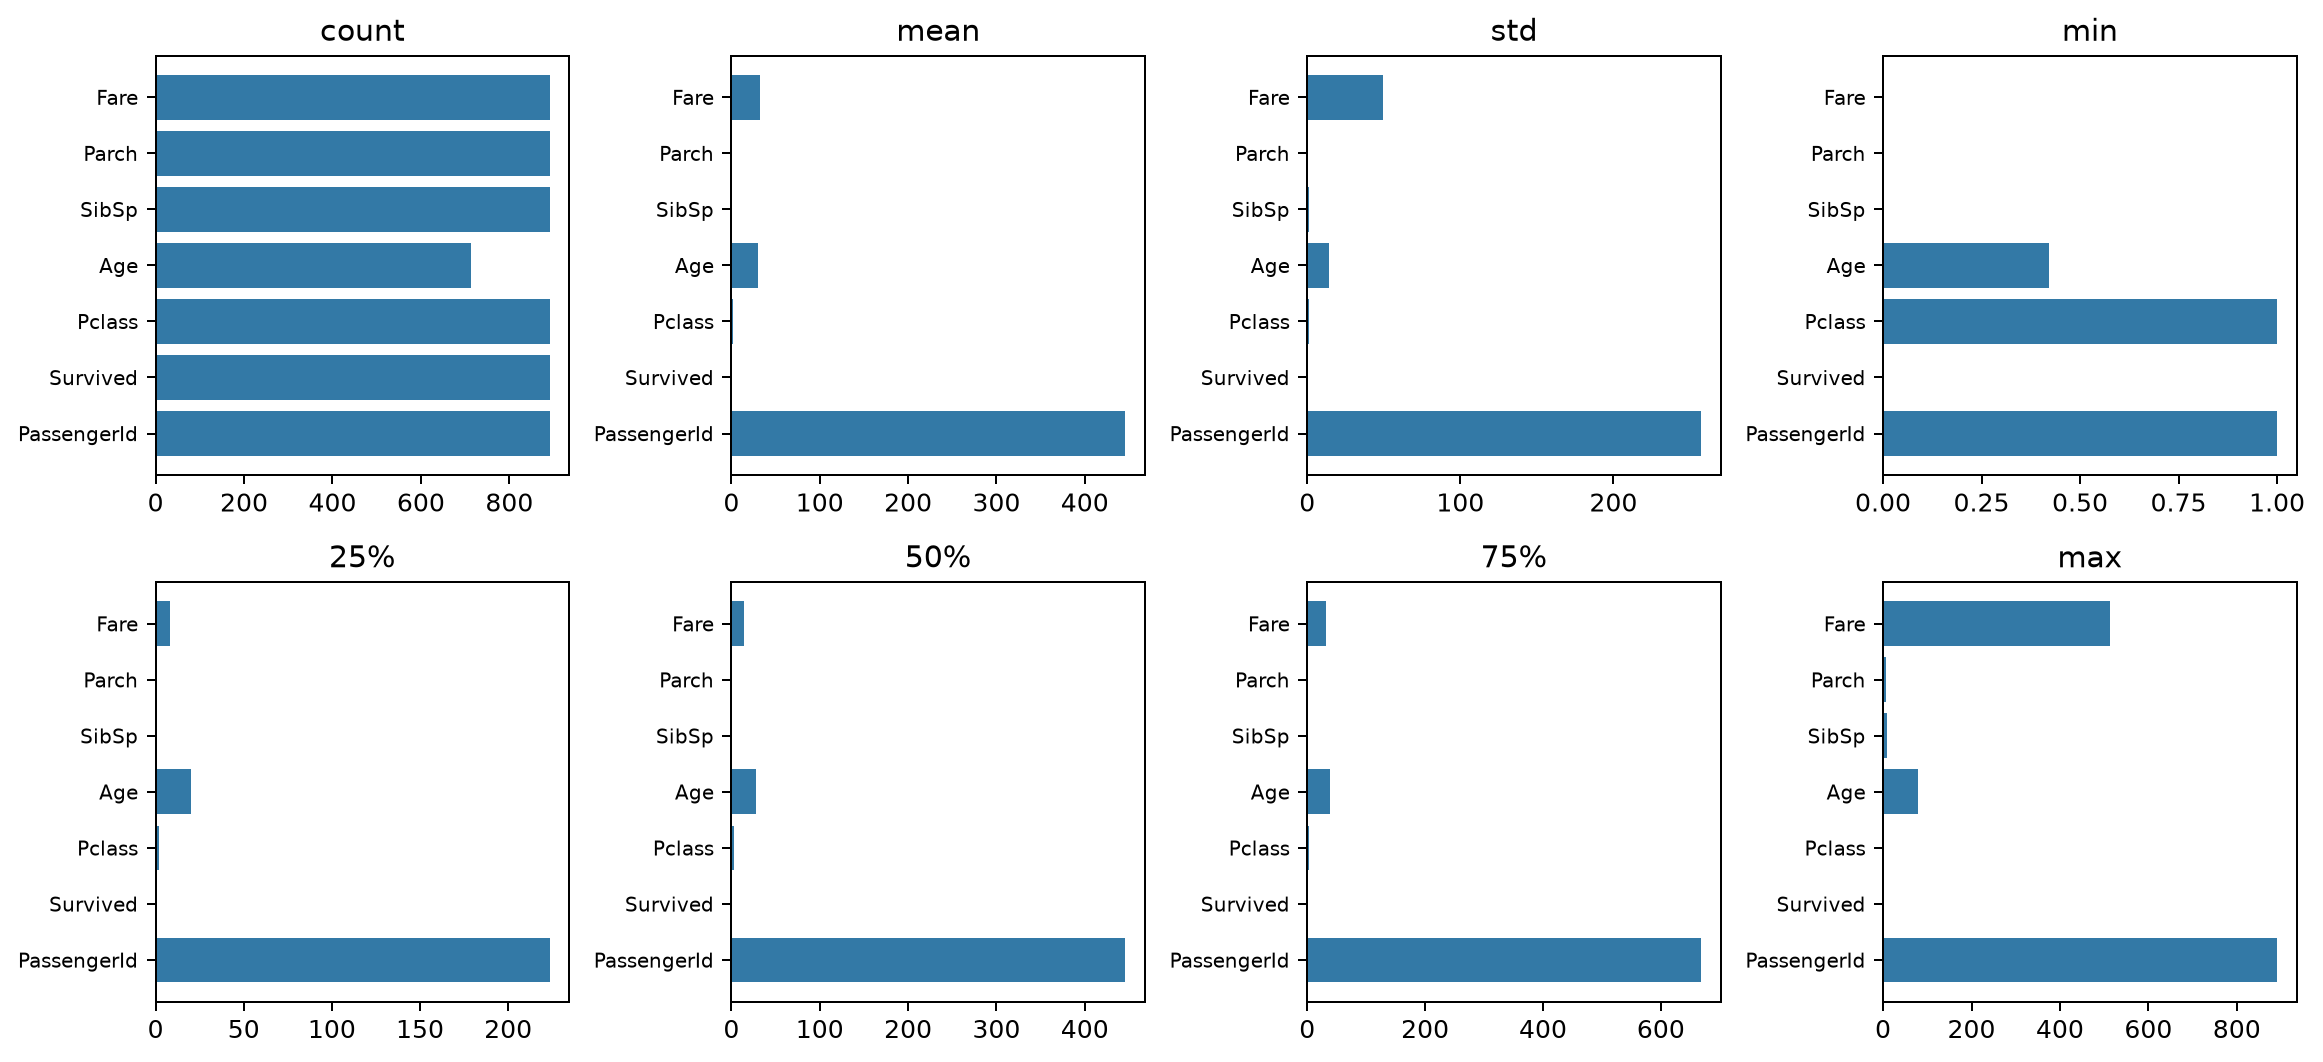
\includegraphics[width=1.0\linewidth]{figures/statistics.png}
\caption{Графическое представление всех восьми статистик}
\end{figure}

\begin{figure}[H]
\centering
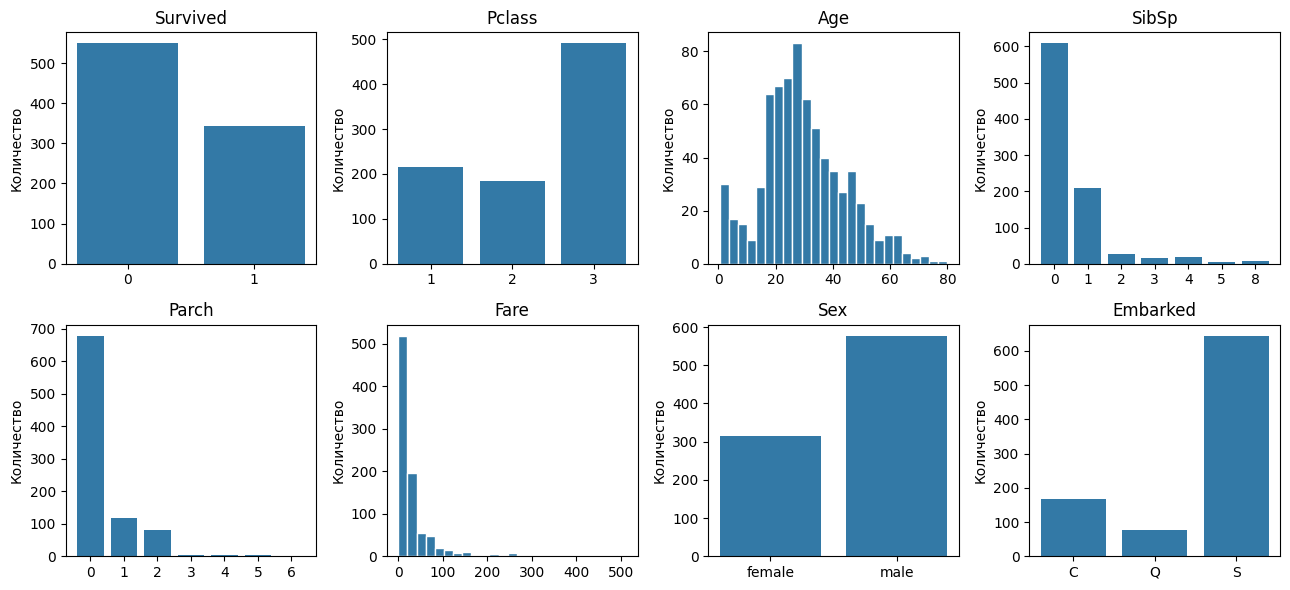
\includegraphics[width=1.0\linewidth]{figures/distributions.png}
\caption{Распределения исходных признаков и целевой переменной}
\end{figure}

Исследована полная сетка: $\alpha\in\{0.01,0.1,0.5,1\}$, $T\in\{10,100,1000\}$ и два оптимизатора, всего 24 модели. Положительный класс - выжившие. Метрики вычислены по формулам:
\[
 A=\frac{TP+TN}{n},\quad P=\frac{TP}{TP+FP},\quad
 R=\frac{TP}{TP+FN},\quad F_1=\frac{2PR}{P+R}.
\]

\begin{table}[H]
\centering
\caption{Градиентный спуск: метрики на тестовой части}
\small
\begin{tabular}{lrrrrrrr}
\toprule
$\alpha$ & $T_{max}$ & $T_{fact}$ & Accuracy & Precision & Recall & F1 & Log loss \\
\midrule
0.01 & 10 & 10 & 0.6461 & 0.7778 & 0.1029 & 0.1818 & 0.6830 \\
0.01 & 100 & 100 & 0.6517 & 0.8000 & 0.1176 & 0.2051 & 0.6252 \\
0.01 & 1000 & 1000 & 0.7247 & 0.8065 & 0.3676 & 0.5051 & 0.5295 \\
0.1 & 10 & 10 & 0.6517 & 0.8000 & 0.1176 & 0.2051 & 0.6244 \\
0.1 & 100 & 100 & 0.7247 & 0.8065 & 0.3676 & 0.5051 & 0.5294 \\
0.1 & 1000 & 1000 & 0.8146 & 0.7966 & 0.6912 & 0.7402 & 0.4410 \\
0.5 & 10 & 10 & 0.6798 & 0.7895 & 0.2206 & 0.3448 & 0.5586 \\
0.5 & 100 & 100 & 0.8146 & 0.8182 & 0.6618 & 0.7317 & 0.4585 \\
0.5 & 1000 & 1000 & 0.8034 & 0.7705 & 0.6912 & 0.7287 & 0.4235 \\
1 & 10 & 10 & 0.7247 & 0.8065 & 0.3676 & 0.5051 & 0.5286 \\
1 & 100 & 100 & 0.8146 & 0.7966 & 0.6912 & 0.7402 & 0.4409 \\
1 & 1000 & 1000 & 0.7921 & 0.7541 & 0.6765 & 0.7132 & 0.4228 \\
\bottomrule
\end{tabular}
\end{table}

\begin{table}[H]
\centering
\caption{Метод Ньютона: метрики на тестовой части}
\small
\begin{tabular}{lrrrrrrr}
\toprule
$\alpha$ & $T_{max}$ & $T_{fact}$ & Accuracy & Precision & Recall & F1 & Log loss \\
\midrule
0.01 & 10 & 10 & 0.7978 & 0.7500 & 0.7059 & 0.7273 & 0.6516 \\
0.01 & 100 & 100 & 0.8034 & 0.7619 & 0.7059 & 0.7328 & 0.4785 \\
0.01 & 1000 & 1000 & 0.7921 & 0.7541 & 0.6765 & 0.7132 & 0.4228 \\
0.1 & 10 & 10 & 0.8034 & 0.7619 & 0.7059 & 0.7328 & 0.4757 \\
0.1 & 100 & 100 & 0.7921 & 0.7541 & 0.6765 & 0.7132 & 0.4228 \\
0.1 & 1000 & 161 & 0.7921 & 0.7541 & 0.6765 & 0.7132 & 0.4228 \\
0.5 & 10 & 10 & 0.7921 & 0.7541 & 0.6765 & 0.7132 & 0.4228 \\
0.5 & 100 & 25 & 0.7921 & 0.7541 & 0.6765 & 0.7132 & 0.4228 \\
0.5 & 1000 & 25 & 0.7921 & 0.7541 & 0.6765 & 0.7132 & 0.4228 \\
1 & 10 & 5 & 0.7921 & 0.7541 & 0.6765 & 0.7132 & 0.4228 \\
1 & 100 & 5 & 0.7921 & 0.7541 & 0.6765 & 0.7132 & 0.4228 \\
1 & 1000 & 5 & 0.7921 & 0.7541 & 0.6765 & 0.7132 & 0.4228 \\
\bottomrule
\end{tabular}
\end{table}

\begin{figure}[H]
\centering
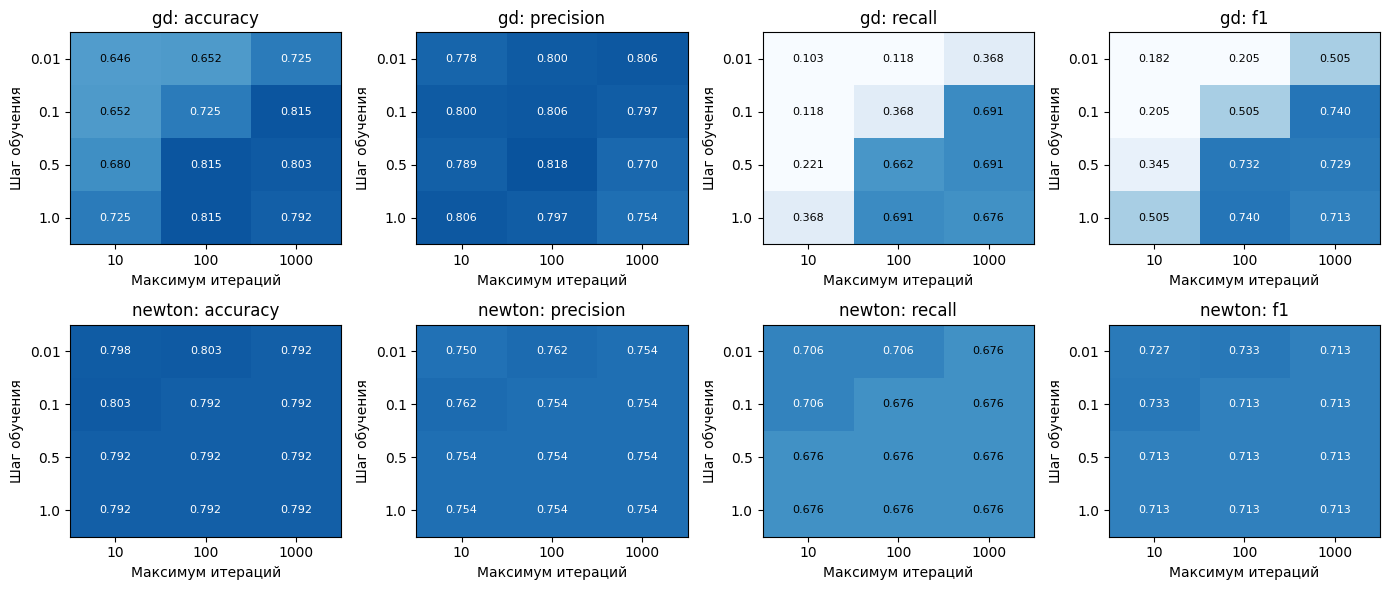
\includegraphics[width=1.0\linewidth]{figures/hyperparameters.png}
\caption{Все четыре метрики для каждой комбинации гиперпараметров}
\end{figure}
Основным критерием выбран F1; при равенстве сравниваются accuracy, меньшая test log loss и меньшее число итераций. Лучший F1=0.740157 получен у GD при $\alpha=0.1$, $T=1000$ и при $\alpha=1$, $T=100$

Матрица ошибок выбранной конфигурации: TN=98, FP=12, FN=21, TP=47. Правильно классифицированы 145 из 178 пассажиров. Из 68 выживших модель обнаружила 47, пропустила 21; 12 невыживших ошибочно отнесены к выжившим.

\begin{figure}[H]
\centering

\includegraphics[width=0.60\linewidth]{figures/confusion.png}
\caption{Матрица ошибок выбранной конфигурации GD}
\end{figure}

\begin{table}[H]
\centering
\caption{Примеры предсказаний на тестовой части}
\small
\begin{tabular}{lrrr}
\toprule
PassengerId & Истинный класс & $p(y=1)$ & Прогноз \\
\midrule
95 & 0 & 0.0485 & 0 \\
235 & 0 & 0.3160 & 0 \\
618 & 0 & 0.5303 & 1 \\
387 & 0 & 0.0632 & 0 \\
358 & 0 & 0.7390 & 1 \\
\bottomrule
\end{tabular}
\end{table}

\section{Примеры использования метода}

В задаче титаника логистическая регрессия позволяет оценить вероятность выживания по классу билета, полу, возрасту, числу родственников и стоимости проезда. Выход модели можно использовать для бинарного решения при заданном пороге; коэффициенты позволяют интерпретировать изменение шансов при фиксированных остальных признаках.

Аналогичная постановка подходит для классификации писем на спам и обычные сообщения, для оценки вероятности ухода клиента или покупки товара. Метод удобен, когда нужна вероятность бинарного события и простая интерпретируемая модель

\section{Сравнение методов}

\subsection{Сравнительный анализ методов}

Оба оптимизатора обучают одну и ту же модель с одной и той же log loss. Различаются направление обновления, скорость сходимости и количество итераций

\begin{figure}[H]
\centering
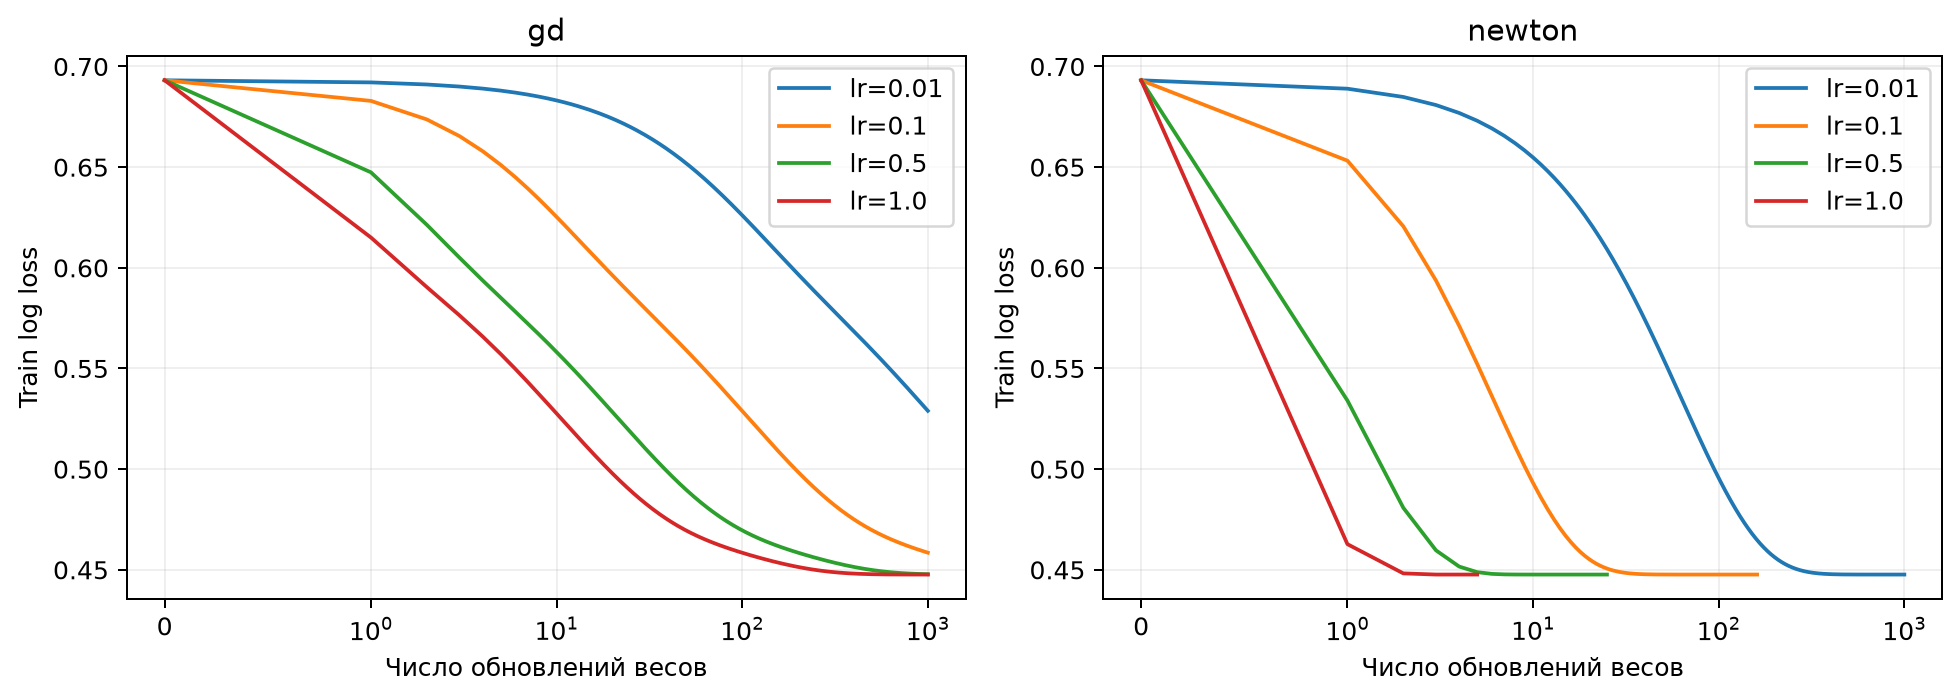
\includegraphics[width=1.0\linewidth]{figures/convergence.png}
\caption{Зависимость train log loss от числа обновлений весов}
\end{figure}

\subsection{Примеры лучшего использования каждого метода}

Градиентный спуск целесообразен для большого числа признаков, когда построение гессиана затратно, и когда важны простота реализации и небольшая дополнительная память. Его ограничения - необходимость выбора шага и потенциально медленное достижение критерия сходимости.

Метод Ньютона удобен для небольших плотных задач, подобных данной матрице из 9 признаков, когда требуется быстро найти минимум log loss. Он использует кривизну функции, но требует хранения гессиана и более дорогой линейной алгебры; при вырожденности требуется устойчивое решение.

\section{Заключение}
В ходе лабораторной работы установлено, что качество предсказания выживания пассажиров Титаник зависит от шага обучения и числа итераций. При малом шаге 0,01 и 10-100 итерациях градиентный спуск обнаруживает лишь около 10-12\% выживших. Увеличение шага или продолжительности обучения позволяет существенно улучшить этот результат.

Наибольшее значение $F_1=0,7402$ получено градиентным спуском при шаге 0,1 и 1000 итерациях, а также при шаге 1 и 100 итерациях. Обе настройки обеспечили долю правильных ответов 81,46\%. При этом дальнейшее увеличение числа итераций не гарантирует улучшения классификации: при шаге 1 переход от 100 к 1000 итерациям уменьшил логарифмическую функцию потерь, но снизил F1 до 0,7132.

Метод Ньютона при шаге 1 достиг сходимости всего за 5 обновлений коэффициентов, однако его F1 составила 0,7132. Следовательно, более быстрое достижение минимума функции потерь не обязательно даёт лучшее качество классификации. Для данного разбиения наиболее удачным сочетанием качества и числа обновлений оказался градиентный спуск с шагом 1 и 100 итерациями.

\clearpage

\section{Приложения}

Для выполнения используются Python 3, NumPy, Pandas и Matplotlib.

\begin{minted}[fontsize=\footnotesize,breaklines,linenos,numbersep=5pt]{python}

import numpy as np
import pandas as pd
import matplotlib.pyplot as plt
from time import perf_counter

df = pd.read_csv('train.csv')

print(f"Размер датасета: {df.shape[0]} строк, {df.shape[1]} столбцов")
print(f"Повторяющиеся строки: {df.duplicated().sum()}")

print("Статистика по датасету:")
stats = df.describe(percentiles=[0.25, 0.5, 0.75]).T
display(stats)

print("Пропущенные значения:")
missing = df.isna().sum().rename('Количество').to_frame()
missing['Доля, %'] = missing['Количество'] / len(df) * 100
display(missing)

fig, axes = plt.subplots(2, 4, figsize=(13, 6))
columns = ['Survived', 'Pclass', 'Age', 'SibSp', 'Parch', 'Fare', 'Sex', 'Embarked']
for ax, col in zip(axes.flat, columns):
    values = df[col].dropna()
    if col in ['Age', 'Fare']:
        ax.hist(values, bins=25, color='#3379a6', edgecolor='white')
    else:
        counts = values.value_counts().sort_index()
        ax.bar(counts.index.astype(str), counts.values, color='#3379a6')
    ax.set_title(col)
    ax.set_ylabel('Количество')
fig.tight_layout()
plt.show()

fig, axes = plt.subplots(2, 4, figsize=(13, 6))
for ax, stat in zip(axes.flat, stats.columns):
    ax.barh(stats.index, stats[stat], color='#3379a6')
    ax.set_title(stat)
    ax.tick_params(axis='y', labelsize=8)
fig.tight_layout()
plt.show()

fig, axes = plt.subplots(1, 2, figsize=(10, 3.5))
nonzero = missing[missing['Количество'] > 0]
axes[0].bar(nonzero.index, nonzero['Доля, %'], color='#bc6940')
axes[0].set_ylabel('Доля пропусков, %')
axes[0].set_title('Пропущенные значения')
class_counts = df.Survived.value_counts().sort_index()
axes[1].bar(['Не выжил (0)', 'Выжил (1)'], class_counts, color=['#bc6940', '#3379a6'])
axes[1].set_ylabel('Количество пассажиров')
axes[1].set_title('Баланс классов')
for i, n in enumerate(class_counts):
    axes[1].text(i, n + 5, str(n), ha='center')
fig.tight_layout()
plt.show()

target_col = 'Survived'
numeric_features = ['Age', 'SibSp', 'Parch', 'Fare']
categorical_features = ['Pclass', 'Sex', 'Embarked']
features = numeric_features + categorical_features

X_full = df[features].copy()
y_full = df[target_col].copy()

print(f"Числовые признаки: {numeric_features}")
print(f"Категориальные признаки: {categorical_features}")

def stratified_split(y, test_size=0.2, random_state=42):
    rng = np.random.default_rng(random_state)
    train, test = [], []
    for label in np.unique(y):
        indices = rng.permutation(np.flatnonzero(y == label))
        n_test = int(round(len(indices) * test_size))
        test.extend(indices[:n_test])
        train.extend(indices[n_test:])
    return rng.permutation(train), rng.permutation(test)

class TitanicPreprocessor:
    numeric = ['Age', 'SibSp', 'Parch', 'Fare']
    categorical = ['Pclass', 'Sex', 'Embarked']

    def fit(self, data):
        self.medians = data[self.numeric].median()
        numeric = data[self.numeric].fillna(self.medians)
        self.means = numeric.mean()
        self.scales = numeric.std(ddof=0).replace(0, 1)
        self.modes = {c: data[c].mode().iloc[0] for c in self.categorical}
        self.categories = {
            c: sorted(data[c].fillna(self.modes[c]).unique())
            for c in self.categorical
        }
        self.feature_names = self.numeric + [
            f'{c}_{value}' for c in self.categorical
            for value in self.categories[c][1:]
        ]
        return self

    def transform(self, data):
        numeric = data[self.numeric].fillna(self.medians)
        parts = [((numeric - self.means) / self.scales).to_numpy(float)]
        for c in self.categorical:
            values = data[c].fillna(self.modes[c])
            if not values.isin(self.categories[c]).all():
                raise ValueError(f'Unknown category in {c}')
            for value in self.categories[c][1:]:
                parts.append((values == value).to_numpy(float)[:, None])
        return np.column_stack(parts)

train_idx, test_idx = stratified_split(df.Survived.to_numpy(), random_state=42)
train, test = df.iloc[train_idx].copy(), df.iloc[test_idx].copy()
assert not set(train.PassengerId) & set(test.PassengerId)
preprocessor = TitanicPreprocessor().fit(train)
X_train, X_test = preprocessor.transform(train), preprocessor.transform(test)
y_train, y_test = train.Survived.to_numpy(), test.Survived.to_numpy()
assert np.isfinite(X_train).all() and np.isfinite(X_test).all()
assert np.allclose(X_train[:, :4].mean(axis=0), 0, atol=1e-12)
assert np.allclose(X_train[:, :4].std(axis=0), 1)
split_info = pd.DataFrame({
    'size': [len(train), len(test)],
    'not_survived': [(y_train == 0).sum(), (y_test == 0).sum()],
    'survived': [(y_train == 1).sum(), (y_test == 1).sum()],
}, index=['train', 'test'])
print(f"Размер обучающей выборки (Train): {X_train.shape[0]} строк")
print(f"Размер тестовой выборки (Test):   {X_test.shape[0]} строк")
display(split_info)
print('Признаки:', preprocessor.feature_names)
print('Медианы train:', preprocessor.medians.to_dict())

class CustomLogisticRegression:
    def __init__(self, learning_rate=0.1, max_iter=1000,
                 optimizer='gd', tol=1e-8):
        if learning_rate <= 0 or max_iter < 1 or optimizer not in ('gd', 'newton'):
            raise ValueError('Invalid hyperparameters')
        self.learning_rate = learning_rate
        self.max_iter = max_iter
        self.optimizer = optimizer
        self.tol = tol

    @staticmethod
    def sigmoid(z):
        z = np.asarray(z, dtype=float)
        out = np.empty_like(z)
        positive = z >= 0
        out[positive] = 1 / (1 + np.exp(-z[positive]))
        exp_z = np.exp(z[~positive])
        out[~positive] = exp_z / (1 + exp_z)
        return out

    @staticmethod
    def log_loss(y, logits):
        return float(np.mean(np.logaddexp(0, logits) - y * logits))

    def fit(self, X, y):
        design = np.column_stack([np.ones(len(X)), X])
        y = np.asarray(y, dtype=float)
        self.weights = np.zeros(design.shape[1])
        self.loss_history = [self.log_loss(y, design @ self.weights)]
        self.n_iter = 0
        self.converged = False
        for _ in range(self.max_iter):
            probabilities = self.sigmoid(design @ self.weights)
            gradient = design.T @ (probabilities - y) / len(y)
            if np.max(np.abs(gradient)) <= self.tol:
                self.converged = True
                break
            if self.optimizer == 'gd':
                direction = gradient
            else:
                curvature = probabilities * (1 - probabilities)
                hessian = design.T @ (design * curvature[:, None]) / len(y)
                direction = np.linalg.pinv(hessian) @ gradient
            self.weights -= self.learning_rate * direction
            loss = self.log_loss(y, design @ self.weights)
            if not np.isfinite(loss):
                raise FloatingPointError('Non-finite training loss')
            self.loss_history.append(loss)
            self.n_iter += 1
        gradient = design.T @ (self.predict_proba(X) - y) / len(y)
        self.gradient_norm = float(np.max(np.abs(gradient)))
        self.converged = self.gradient_norm <= self.tol
        return self

    def decision_function(self, X):
        return self.weights[0] + np.asarray(X) @ self.weights[1:]

    def predict_proba(self, X):
        return self.sigmoid(self.decision_function(X))

    def predict(self, X):
        return (self.predict_proba(X) >= 0.5).astype(int)

    def print_equation(self, feature_names):
        equation = f"z = {self.weights[0]:.4f}"
        for name, weight in zip(feature_names, self.weights[1:]):
            sign = '+' if weight >= 0 else '-'
            equation += f" {sign} {abs(weight):.4f}*{name}"
        print("Логистическая модель в скалярном виде:")
        print(equation)
        print("p(y=1) = 1 / (1 + exp(-z))")

def classification_metrics(y, prediction):
    y, prediction = np.asarray(y), np.asarray(prediction)
    tp = int(np.sum((y == 1) & (prediction == 1)))
    tn = int(np.sum((y == 0) & (prediction == 0)))
    fp = int(np.sum((y == 0) & (prediction == 1)))
    fn = int(np.sum((y == 1) & (prediction == 0)))
    precision = tp / (tp + fp) if tp + fp else 0.0
    recall = tp / (tp + fn) if tp + fn else 0.0
    f1 = 2 * precision * recall / (precision + recall) if precision + recall else 0.0
    return dict(accuracy=(tp + tn) / len(y), precision=precision,
                recall=recall, f1=f1, tp=tp, tn=tn, fp=fp, fn=fn)

LEARNING_RATES = [0.01, 0.1, 0.5, 1.0]
ITERATIONS = [10, 100, 1000]
OPTIMIZERS = ['gd', 'newton']
records, models = [], {}

for learning_rate in LEARNING_RATES:
    for max_iter in ITERATIONS:
        model = CustomLogisticRegression(learning_rate, max_iter, 'gd')
        start = perf_counter()
        model.fit(X_train, y_train)
        elapsed = (perf_counter() - start) * 1000
        y_pred = model.predict(X_test)
        metrics = classification_metrics(y_test, y_pred)
        models[('gd', learning_rate, max_iter)] = model
        records.append(dict(
            optimizer='gd', learning_rate=learning_rate,
            max_iter=max_iter, n_iter=model.n_iter, converged=model.converged,
            gradient_norm=model.gradient_norm, time_ms=elapsed,
            train_log_loss=model.loss_history[-1],
            test_log_loss=model.log_loss(y_test, model.decision_function(X_test)),
            **metrics
        ))

print("Градиентнаый спуск")
results_gd = pd.DataFrame([r for r in records if r['optimizer'] == 'gd'])
display(results_gd[[
    'learning_rate', 'max_iter', 'n_iter', 'accuracy',
    'precision', 'recall', 'f1', 'test_log_loss'
]].round(6))

for learning_rate in LEARNING_RATES:
    for max_iter in ITERATIONS:
        model = CustomLogisticRegression(learning_rate, max_iter, 'newton')
        start = perf_counter()
        model.fit(X_train, y_train)
        elapsed = (perf_counter() - start) * 1000
        y_pred = model.predict(X_test)
        metrics = classification_metrics(y_test, y_pred)
        models[('newton', learning_rate, max_iter)] = model
        records.append(dict(
            optimizer='newton', learning_rate=learning_rate,
            max_iter=max_iter, n_iter=model.n_iter, converged=model.converged,
            gradient_norm=model.gradient_norm, time_ms=elapsed,
            train_log_loss=model.loss_history[-1],
            test_log_loss=model.log_loss(y_test, model.decision_function(X_test)),
            **metrics
        ))

print("Метод Ньютона")
results_newton = pd.DataFrame([r for r in records if r['optimizer'] == 'newton'])
display(results_newton[[
    'learning_rate', 'max_iter', 'n_iter', 'accuracy',
    'precision', 'recall', 'f1', 'test_log_loss'
]].round(6))

summary_df = pd.DataFrame(records)
results = summary_df
ranked = summary_df.sort_values(
    ['f1', 'accuracy', 'test_log_loss', 'max_iter'],
    ascending=[False, False, True, True], kind='stable'
)
best = ranked.iloc[0]
best_model = models[(best.optimizer, float(best.learning_rate), int(best.max_iter))]
y_pred = best_model.predict(X_test)

print("Итоговое сравнение")
display(summary_df[[
    'optimizer', 'learning_rate', 'max_iter', 'n_iter',
    'accuracy', 'precision', 'recall', 'f1', 'test_log_loss'
]].round(6))

print("--- Наилучшая конфигурация ---")
print(f"Метод: {best.optimizer}")
print(f"Коэффициент обучения: {best.learning_rate:g}")
print(f"Количество итераций: {int(best.max_iter)}")
print(f"Признаки: {preprocessor.feature_names}")
best_model.print_equation(preprocessor.feature_names)
print("\nОценки параметров (Вектор B):")
print(f"Свободный член (a): {best_model.weights[0]:.4f}")
for name, weight in zip(preprocessor.feature_names, best_model.weights[1:]):
    print(f"Коэффициент при {name}: {weight:.4f}")
print("-" * 30)
print(f"Accuracy:  {best.accuracy:.5f}")
print(f"Precision: {best.precision:.5f}")
print(f"Recall:    {best.recall:.5f}")
print(f"F1-Score:  {best.f1:.5f}")
print("Первые 5 вероятностей:      ", np.round(best_model.predict_proba(X_test)[:5], 4))
print("Первые 5 предсказаний:      ", y_pred[:5])
print("Первые 5 реальных значений:", y_test[:5])

benchmarks = []
for optimizer in OPTIMIZERS:
    times, counts = [], []
    for repeat in range(7):
        model = CustomLogisticRegression(1.0, 1000, optimizer)
        start = perf_counter()
        model.fit(X_train, y_train)
        times.append((perf_counter() - start) * 1000)
        counts.append(model.n_iter)
    benchmarks.append(dict(optimizer=optimizer, learning_rate=1.0, max_iter=1000,
                           median_time_ms=float(np.median(times)),
                           n_iter=counts[-1], train_log_loss=model.loss_history[-1],
                           gradient_norm=model.gradient_norm, converged=model.converged))
benchmark = pd.DataFrame(benchmarks)
print('\nСравнение времени (медиана 7 запусков):')
display(benchmark)

fig, axes = plt.subplots(2, 4, figsize=(14, 6))
for row, optimizer in enumerate(OPTIMIZERS):
    for col, metric in enumerate(['accuracy', 'precision', 'recall', 'f1']):
        ax = axes[row, col]
        matrix = results[results.optimizer == optimizer].pivot(
            index='learning_rate', columns='max_iter', values=metric)
        ax.imshow(matrix, vmin=0.3, vmax=0.9, cmap='Blues', aspect='auto')
        ax.set_xticks(range(len(ITERATIONS)), ITERATIONS)
        ax.set_yticks(range(len(LEARNING_RATES)), LEARNING_RATES)
        ax.set_title(f'{optimizer}: {metric}')
        ax.set_xlabel('Максимум итераций')
        ax.set_ylabel('Шаг обучения')
        for i in range(len(LEARNING_RATES)):
            for j in range(len(ITERATIONS)):
                v = matrix.iloc[i, j]
                ax.text(j, i, f'{v:.3f}', ha='center', va='center',
                        color='white' if v > 0.7 else 'black', fontsize=8)
fig.tight_layout()
plt.show()

fig, axes = plt.subplots(1, 2, figsize=(11, 4))
for ax, optimizer in zip(axes, OPTIMIZERS):
    for lr in LEARNING_RATES:
        model = models[(optimizer, lr, 1000)]
        ax.plot(np.arange(len(model.loss_history)), model.loss_history, label=f'lr={lr}')
    ax.set_xscale('symlog', linthresh=1)
    ax.set_xlabel('Число обновлений весов')
    ax.set_ylabel('Train log loss')
    ax.set_title(optimizer)
    ax.legend()
    ax.grid(alpha=0.2)
fig.tight_layout()
plt.show()

prediction = best_model.predict(X_test)
metrics = classification_metrics(y_test, prediction)
confusion = np.array([[metrics['tn'], metrics['fp']], [metrics['fn'], metrics['tp']]])
fig, ax = plt.subplots(figsize=(5, 4))
ax.imshow(confusion, cmap='Blues')
ax.set_xticks([0, 1], ['Не выжил', 'Выжил'])
ax.set_yticks([0, 1], ['Не выжил', 'Выжил'])
ax.set_xlabel('Предсказанный класс')
ax.set_ylabel('Истинный класс')
ax.set_title('Матрица ошибок наилучшей конфигурации')
for (i, j), value in np.ndenumerate(confusion):
    ax.text(j, i, str(value), ha='center', va='center', fontsize=16,
            color='white' if value > confusion.max() / 2 else 'black')
fig.tight_layout()
plt.show()
\end{minted}

\end{document}